\subsection{XMPP Modeling in UPPAAL}

This section details our formal model of the XMPP protocol, developed using UPPAAL. This model specifically represents the communication flow between a sender (\texttt{Sender}) and multiple receivers (\texttt{Receiver}), all mediated by a central server (\texttt{Server}). The design captures the core elements of XMPP communication, including the critical stream establishment process, the exchange of messages with varying types and priorities, and fundamental error handling mechanisms \cite{meijer2005jabber,rfc6120}.

\subsubsection{Component Description}

\paragraph{Sender}
The \texttt{Sender} component is tasked with initiating communication and transmitting messages to receivers through the server \cite{meijer2005jabber}. Its primary objective is to send messages to receivers via the server. A key feature is the \texttt{sendQueue}, which stores messages along with their respective priorities, reflecting XMPP's capability to manage diverse message types and their importance \cite{smith2009xmpp}. The \texttt{Sender}'s behavior includes initializing the system and sending messages sequentially, adhering to priority order \cite{waher2015learning}. It also implements XMPP's reliability mechanisms by resending messages in case of an error using the \texttt{retryMessage} functionality \cite{rfc6120}. Furthermore, it closes the stream with each receiver after all messages have been sent, utilizing the \texttt{FIRST\_CST\_MESSAGE} to follow the XMPP stream termination process \cite{meijer2005jabber}. Functions like \texttt{sendNextMessage}, \texttt{retryMessage}, and \texttt{isNextMessageType} are employed to manage message sending and resending, simulating the logic commonly found in XMPP clients \cite{adams2002xep}.

\begin{figure}[h]
\centering
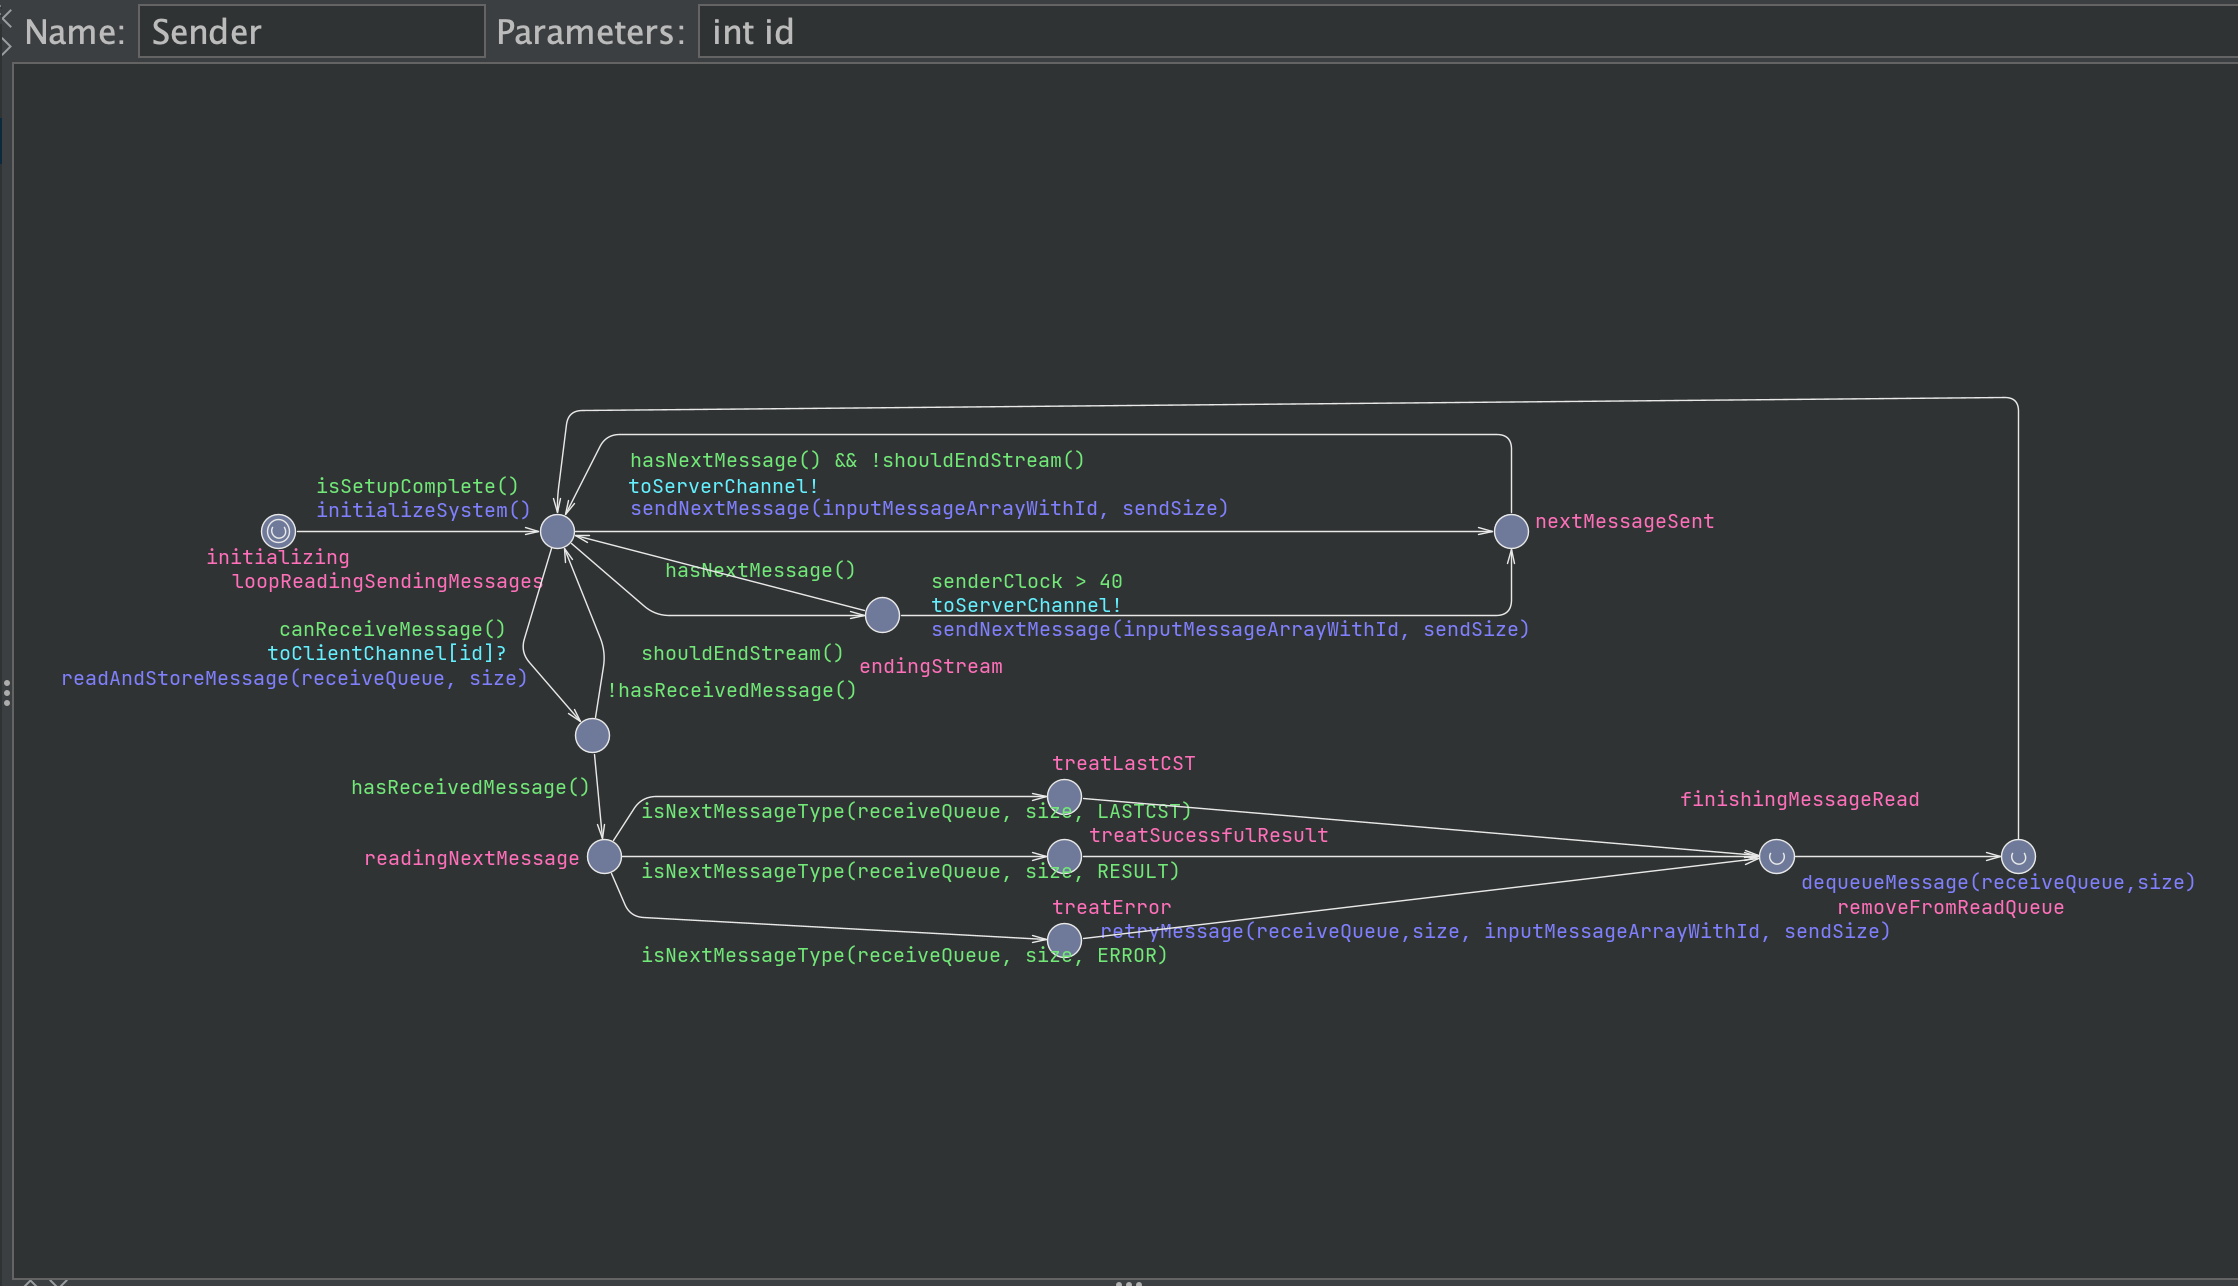
\includegraphics[width=0.8\textwidth]{V3 - Caio Mello - Formal Modeling and Verification of the XMPP Protocol using UPPAAL/img/sender.png}
\caption{Sender Model}
\label{fig:sender}
\end{figure}

\paragraph{Receiver}
The \texttt{Receiver} component embodies XMPP clients responsible for receiving and processing messages \cite{meijer2005jabber}. Its main objective is to receive messages from the sender via the server. Messages are stored in a \texttt{receiveQueue}, which models the message handling capabilities typical of XMPP clients \cite{adams2002xep}. The \texttt{Receiver}'s behavior involves initiating the stream by responding to the \texttt{Sender}, thus implementing the XMPP handshake process \cite{rfc6120}. It receives and processes messages based on their type (e.g., \texttt{IQ\_SET\_MESSAGE}, \texttt{IQ\_GET\_MESSAGE}, \texttt{NORMAL\_MESSAGE}), mirroring the varied XMPP stanza types \cite{smith2009xmpp}. The model also simulates processing errors with a configurable \texttt{errorProbability}, accounting for potential failures in real XMPP systems \cite{waher2015learning}. Following the XMPP response pattern for IQ stanzas, it responds to the sender with either \texttt{RESULT\_MESSAGE} (success) or \texttt{ERROR\_MESSAGE} \cite{rfc6120}. Finally, the \texttt{Receiver} closes the stream upon receiving \texttt{FIRST\_CST\_MESSAGE}, responding with \texttt{LAST\_CST\_MESSAGE}, thereby implementing the XMPP stream termination protocol \cite{meijer2005jabber}.

\begin{figure}[h]
 \centering
 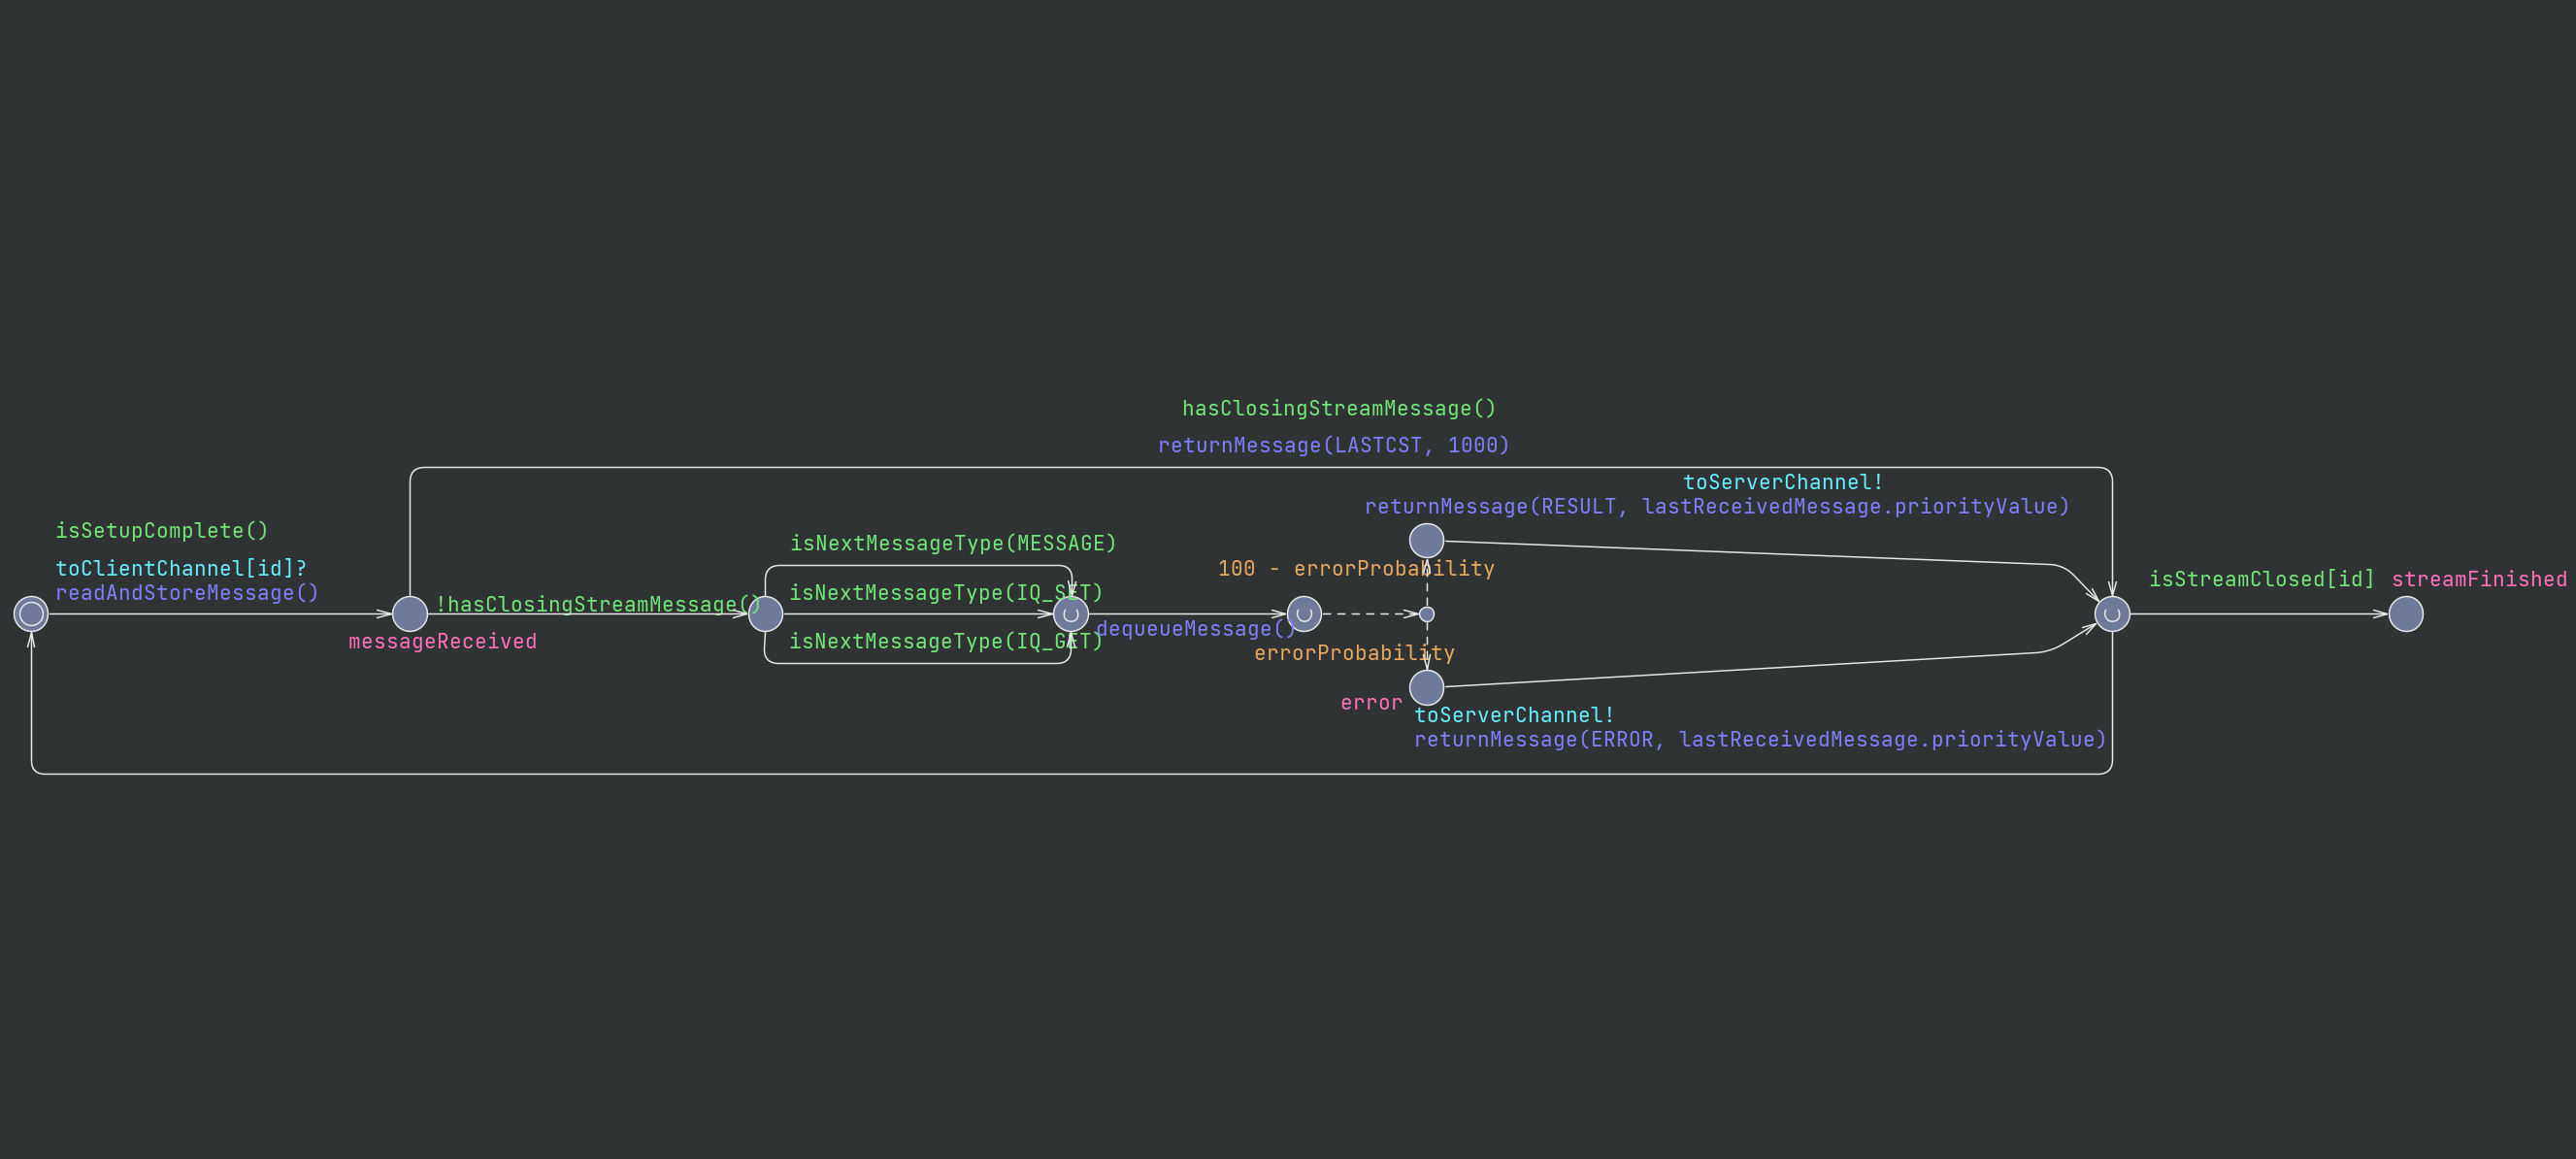
\includegraphics[width=0.8\textwidth]{V3 - Caio Mello - Formal Modeling and Verification of the XMPP Protocol using UPPAAL/img/receiver.png} 
 \caption{Receiver Model}
 \label{fig:receiver}
\end{figure}

\paragraph{Server}
The \texttt{Server} component serves as the intermediary for communication between \texttt{Senders} and \texttt{Receivers}, reflecting the central role of XMPP servers \cite{meijer2005jabber}. Its primary objective is to mediate communication. It uses a \texttt{buffer} to store messages in transit, thereby modeling the store-and-forward mechanism characteristic of XMPP servers \cite{smith2009xmpp}. The \texttt{Server}'s behavior includes receiving messages from the \texttt{Sender} and forwarding them to the correct \texttt{Receiver}, which implements the essential XMPP routing logic \cite{rfc6120}. Conversely, it also receives messages from the \texttt{Receiver} and forwards them to the \texttt{Sender}, thus completing the bidirectional communication flow \cite{meijer2005jabber}. Ultimately, the \texttt{Server} manages the entire message flow, ensuring correct delivery, a critical responsibility of XMPP servers \cite{waher2015learning}.

\begin{figure}[h]
 \centering
 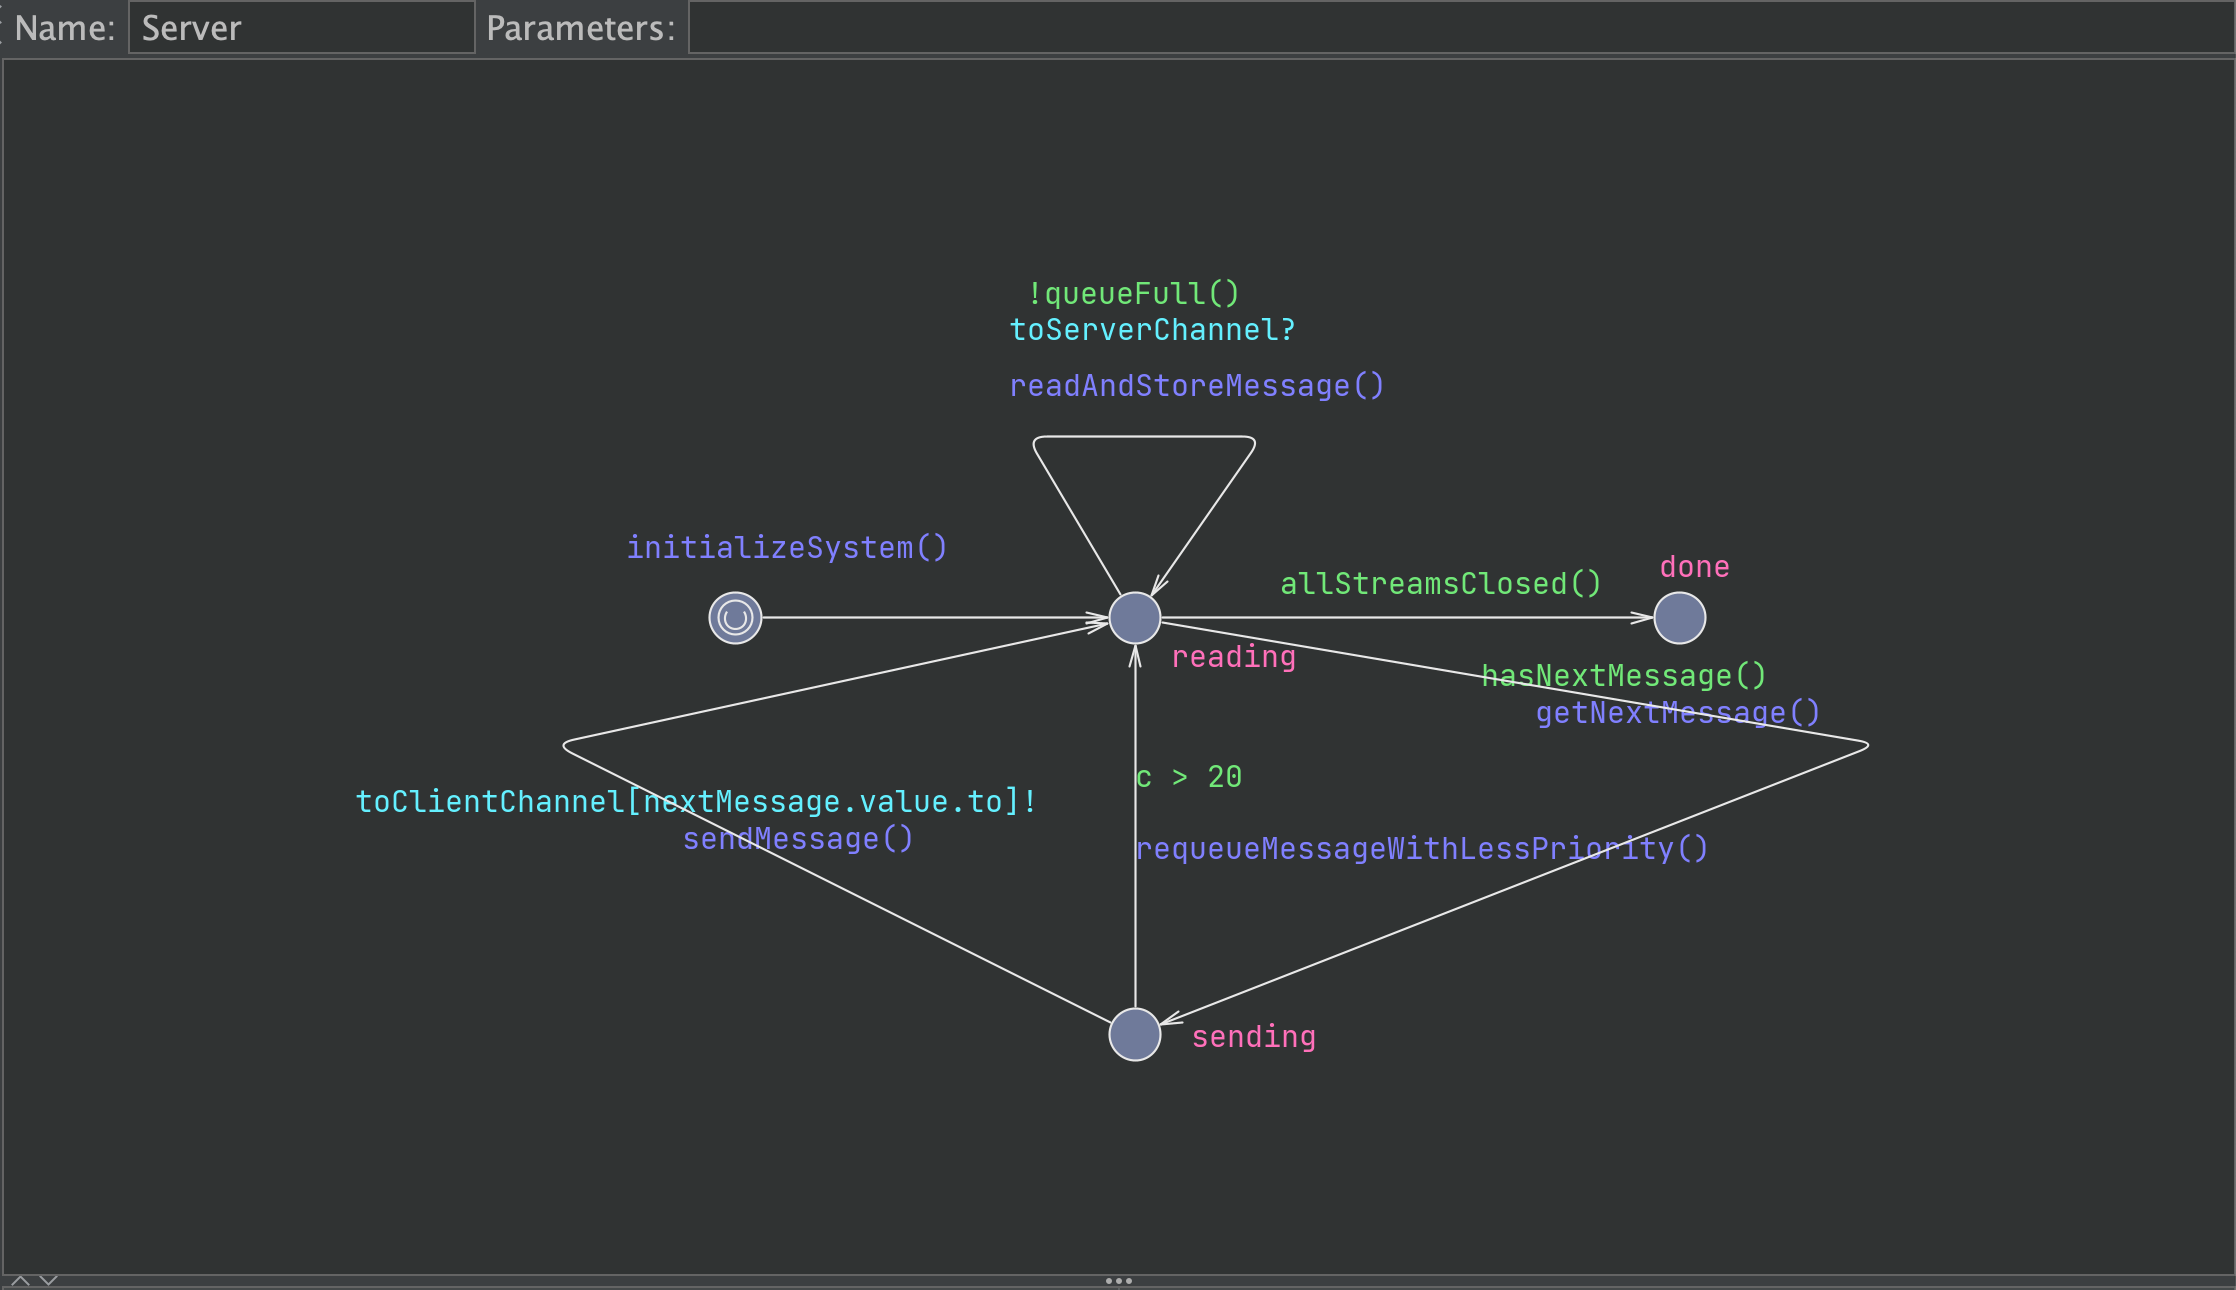
\includegraphics[width=0.8\textwidth]{V3 - Caio Mello - Formal Modeling and Verification of the XMPP Protocol using UPPAAL/img/server.png} 
 \caption{Server Model}
 \label{fig:server}
\end{figure}

\paragraph{SenderStreamSetup and ReceiverStreamSetup}
These two components are dedicated to handling the establishment of XML streams between communicating entities, which is a critical phase of the XMPP protocol \cite{rfc6120}. The \texttt{SenderStreamSetup} component's objective is to establish the stream between the \texttt{Sender} and each \texttt{Receiver}. Its behavior involves sending the \texttt{ISH\_MESSAGE} to initiate the handshake, corresponding to the opening XML stream tag in XMPP \cite{meijer2005jabber}. It then waits for the \texttt{RSH\_MESSAGE} response from the \texttt{Receiver}, modeling the response stream header in XMPP \cite{rfc6120}, and subsequently finalizes the stream establishment process, thereby enabling subsequent message exchange \cite{waher2015learning}. Conversely, the \texttt{ReceiverStreamSetup} component's objective is to establish the stream by responding to the \texttt{Sender}. Its behavior entails waiting for the \texttt{ISH\_MESSAGE} from the \texttt{Sender}, representing the waiting state of XMPP clients \cite{adams2002xep}. It then responds with \texttt{RSH\_MESSAGE} to complete the handshake, corresponding to the XMPP stream response \cite{rfc6120}, and finally formalizes the stream establishment process from the receiver's perspective \cite{meijer2005jabber}.

\begin{figure}[h]
 \centering
 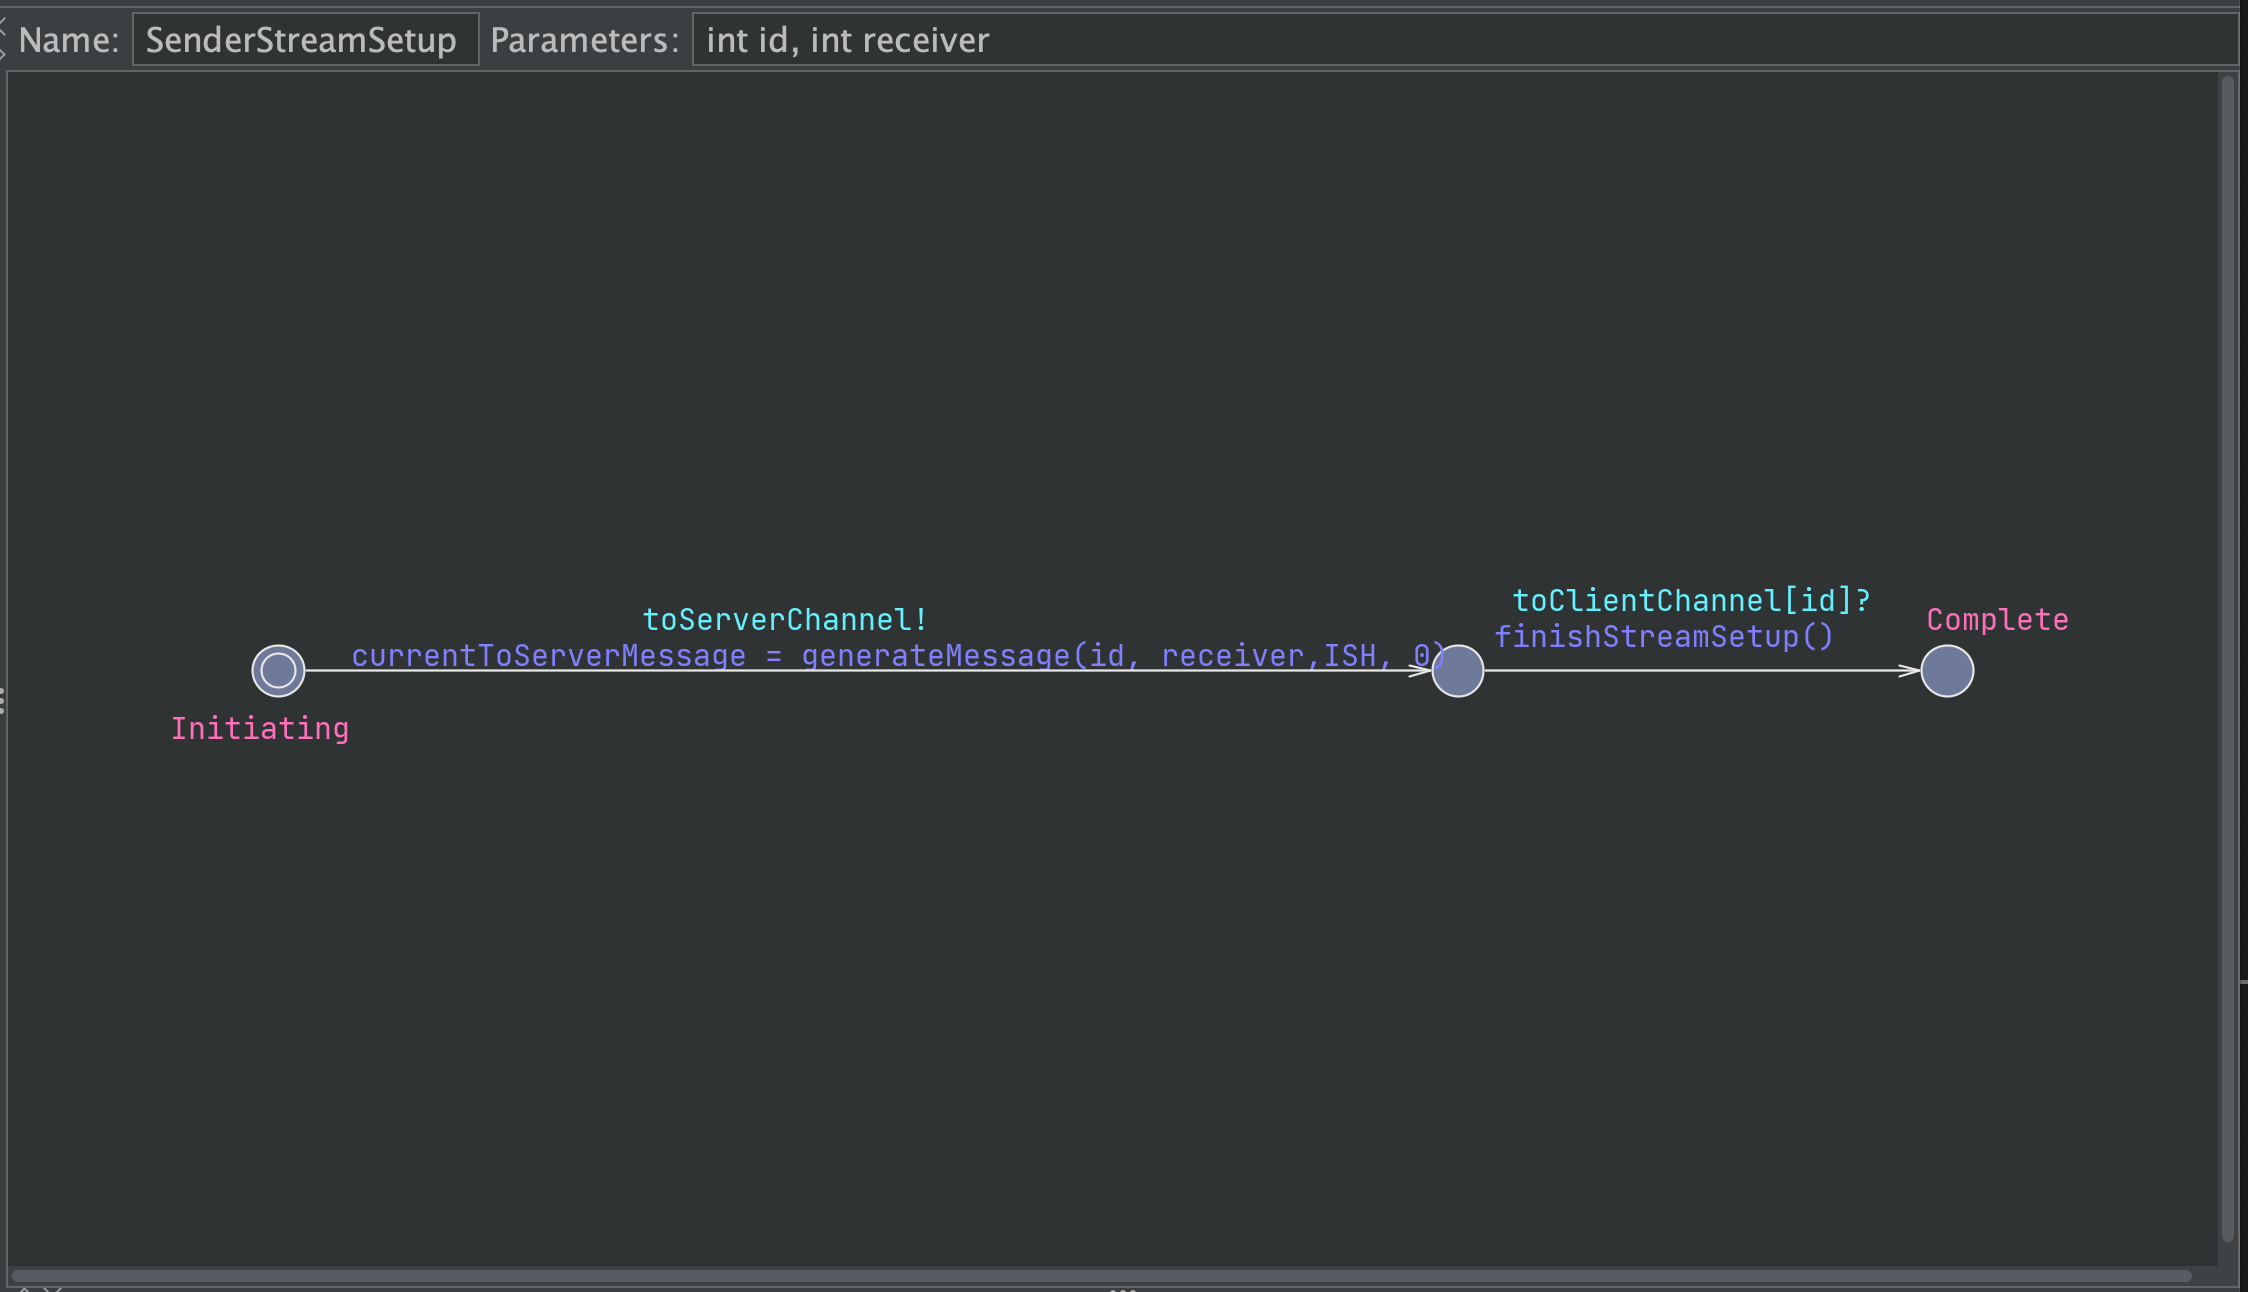
\includegraphics[width=0.8\textwidth]{V3 - Caio Mello - Formal Modeling and Verification of the XMPP Protocol using UPPAAL/img/senderStreamSetup.png} 
 \caption{Sender Stream Setup Model}
 \label{fig:senderStreamSetup}
\end{figure}

\begin{figure}[h]
 \centering
 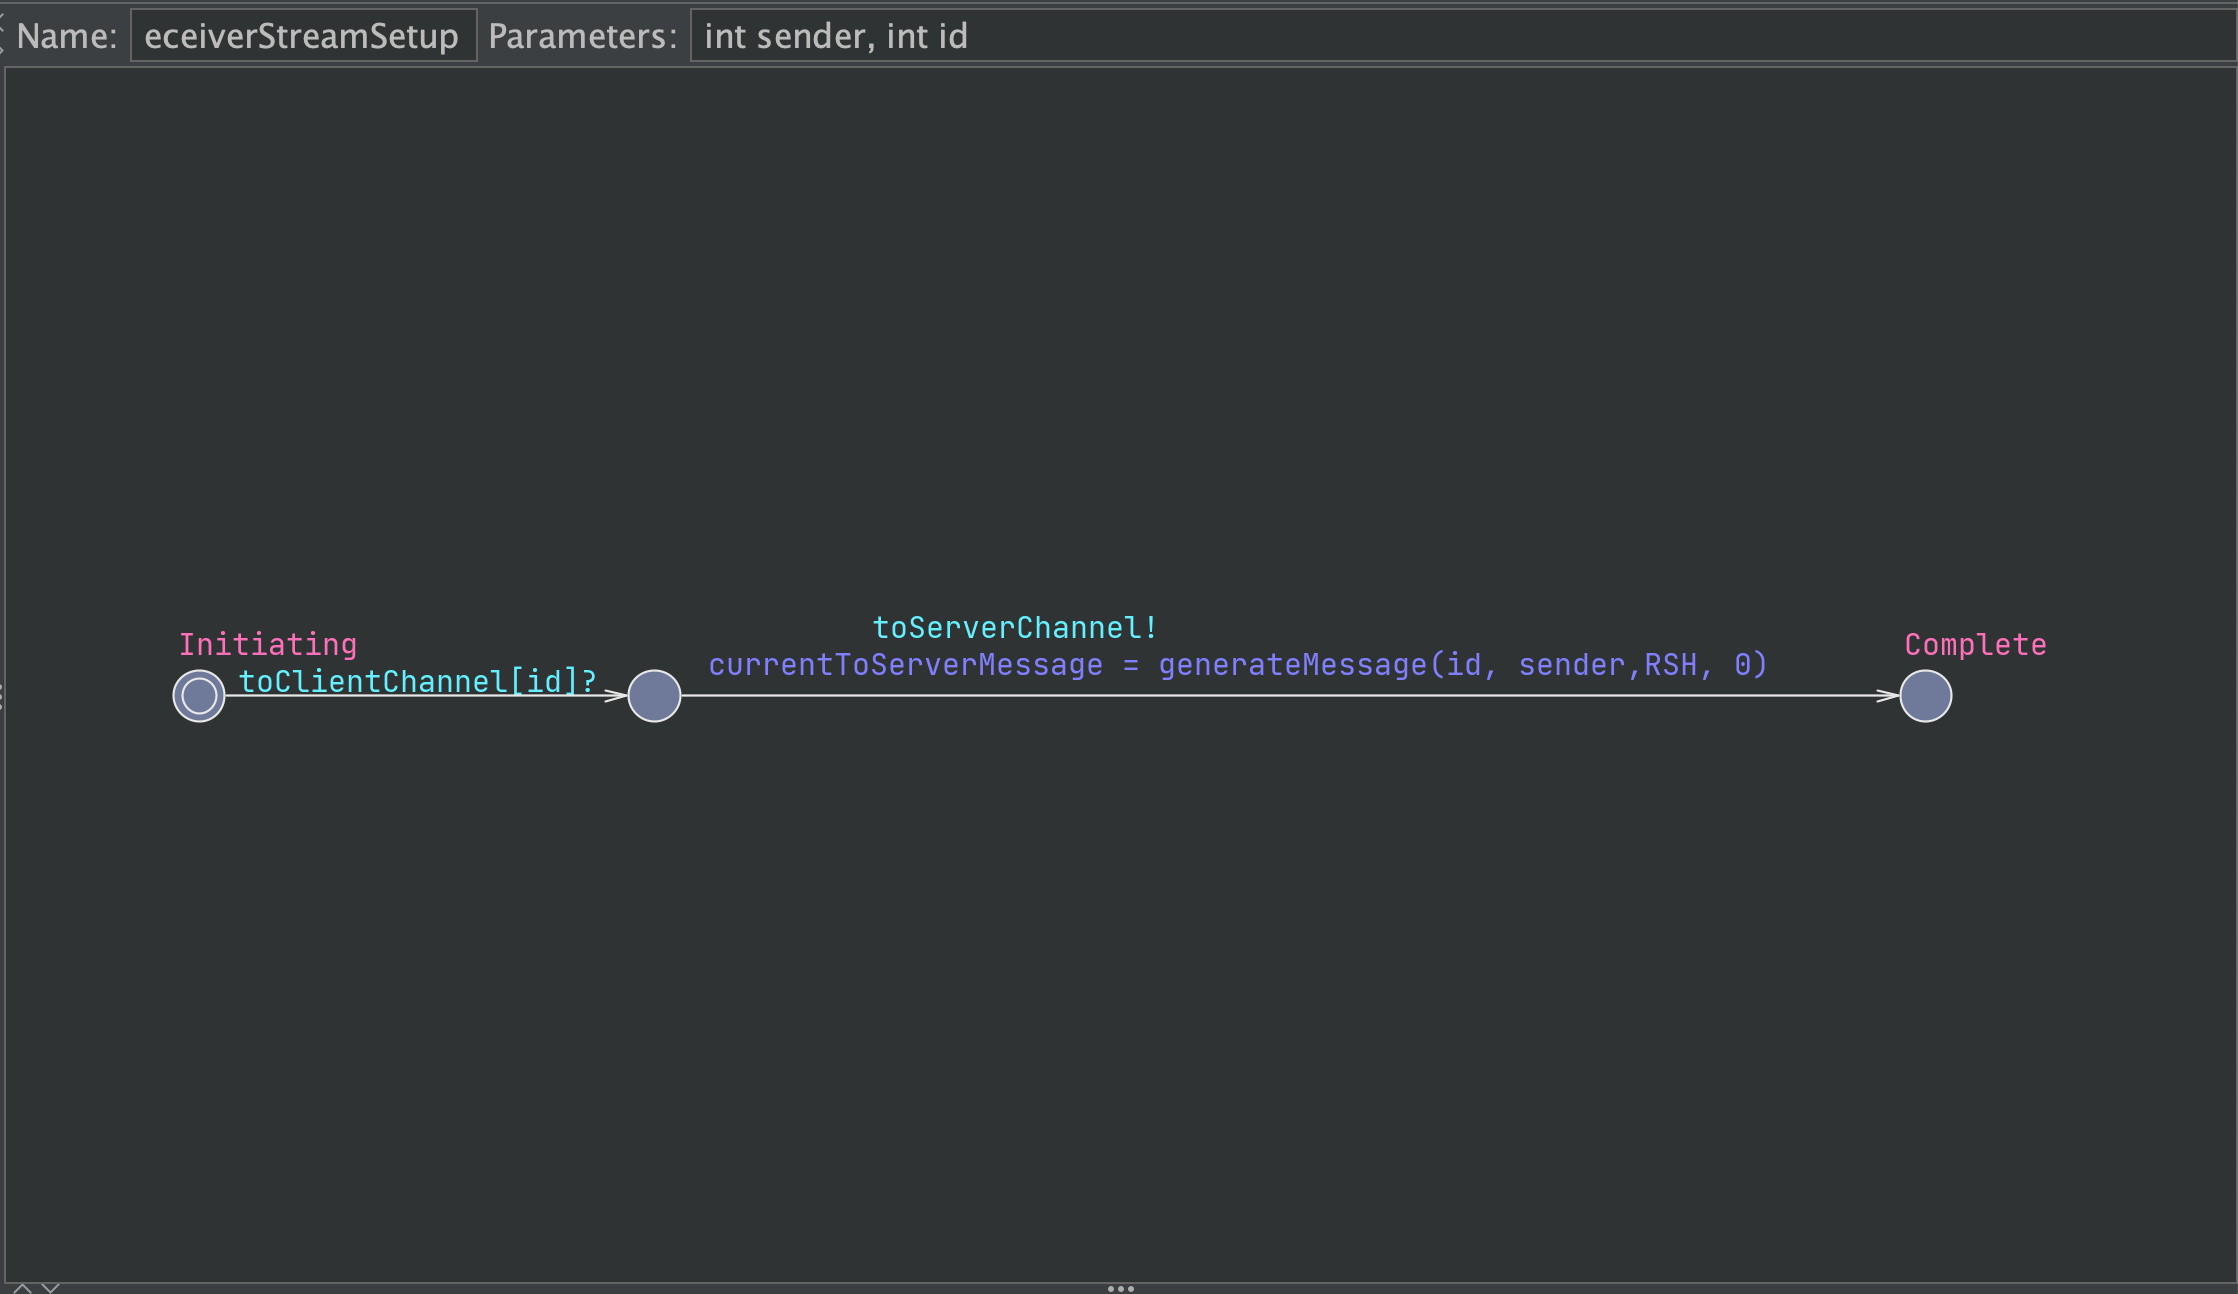
\includegraphics[width=0.8\textwidth]{V3 - Caio Mello - Formal Modeling and Verification of the XMPP Protocol using UPPAAL/img/receiverStreamSetup.png} 
 \caption{Receiver Stream Setup Model}
 \label{fig:receiverStreamSetup}
\end{figure}

\subsubsection{Communication Flow}
The communication flow within our XMPP model meticulously adheres to the standard XMPP protocol sequence \cite{rfc6120,meijer2005jabber}. This sequence begins with Stream Establishment, where \texttt{SenderStreamSetup} and \texttt{ReceiverStreamSetup} exchange \texttt{ISH\_MESSAGE} and \texttt{RSH\_MESSAGE} to initiate communication, effectively modeling the XMPP stream negotiation process \cite{rfc6120}. Next, during Message Sending, the \texttt{Sender} transmits messages from its \texttt{sendQueue} to the \texttt{Server}, representing the client-to-server communication inherent in XMPP \cite{meijer2005jabber}. The Routing phase involves the \texttt{Server} receiving these messages, temporarily storing them in its \texttt{buffer}, and then forwarding them to the designated \texttt{Receiver}, thereby implementing the XMPP server's core routing functionality \cite{smith2009xmpp}. Following this, Processing and Response occurs as the \texttt{Receiver} processes the received message and sends a response (either \texttt{RESULT\_MESSAGE} for success or \texttt{ERROR\_MESSAGE} for an issue) back to the \texttt{Server}, modeling the XMPP response mechanism \cite{rfc6120}. The Response Delivery phase then sees the \texttt{Server} forwarding this response back to the \texttt{Sender}, completing the communication cycle \cite{meijer2005jabber}. In cases of error ( \texttt{ERROR\_MESSAGE}), the Resending mechanism triggers the \texttt{Sender} to resend the message, implementing XMPP's error handling and reliability features \cite{waher2015learning}. Finally, Termination is initiated by the \texttt{Sender} sending \texttt{FIRST\_CST\_MESSAGE} to close the stream, to which the \texttt{Receiver} responds with \texttt{LAST\_CST\_MESSAGE} and then terminates its connection, following the specified XMPP stream closure protocol \cite{rfc6120}.

\subsubsection{Modeling Decisions and Simplifications}
Our UPPAAL model incorporates several key aspects of XMPP while intentionally making necessary simplifications to manage overall complexity \cite{larsen1997uppaal,clarke1997model}. We explicitly model different XMPP Message Types ( \texttt{IQ}, \texttt{Message}, \texttt{Presence}) with varying priorities, reflecting the diverse stanza types found in XMPP \cite{smith2009xmpp}. We also include basic Error Handling and recovery mechanisms, though these are simplified compared to the comprehensive XMPP error handling specification \cite{rfc6120}. Furthermore, we model the core Stream Establishment and Termination processes, which are fundamental to XMPP communication \cite{meijer2005jabber}. Regarding Simplifications, we abstract away granular details of XML parsing and formatting, prioritizing the modeling of protocol-level behavior \cite{clarke1997model}. We omit certain advanced XMPP features, such as TLS negotiation, SASL authentication, and server-to-server communication, to keep the model manageable \cite{baier2008principles}. Additionally, we use a simplified addressing scheme instead of a full JID implementation \cite{adams2002xep}. Despite these simplifications, our model effectively captures the essential behavior of XMPP communication, providing a solid foundation for the formal verification of key protocol properties \cite{clarke1997model,larsen1997uppaal}.

\subsubsection{UPPAAL Representation}
Within UPPAAL, our XMPP model is represented as a network of timed automata, with each logical component ( \texttt{Sender}, \texttt{Receiver}, \texttt{Server}, \texttt{SenderStreamSetup}, \texttt{ReceiverStreamSetup}) being defined as a distinct template \cite{larsen1997uppaal}. These templates include specific locations that represent the different operational states of each component, while edges symbolize transitions between these states, triggered by message exchanges or internal actions \cite{bengtsson2003timed}. The model incorporates several key features designed to capture the real-time aspects inherent in XMPP \cite{alur1994theory,larsen1997uppaal}. \texttt{Clocks} are used to model crucial timeouts and delays in message processing and delivery, accurately reflecting the timing considerations within XMPP systems \cite{waher2015learning}. \texttt{Guards} serve as conditions on transitions, ensuring adherence to the correct protocol sequence, such as verifying message types or buffer availability \cite{bengtsson2003timed}. \texttt{Synchronization Channels} are employed to model the exchange of messages between components, effectively representing the communication channels found in XMPP \cite{larsen1997uppaal}. Lastly, \texttt{Global Variables} are utilized to track overarching system states, manage message queues, and store configuration parameters like the number of clients and the error probability \cite{behrmann2004tutorial}.

\subsubsection{System Configuration and Simulation}
To facilitate the analysis and simulation of various XMPP scenarios, we've developed a meta-model that automates the generation of UPPAAL configurations. This meta-model offers flexible control over system parameters, allowing for the configuration of elements such as the number of clients and error probability. It supports the definition of predefined messages in a specific order and enables the generation of random messages with different types and priorities. Crucially, it handles the creation of UPPAAL system declarations with the appropriate component instances, simplifying the setup process. This meta-model significantly streamlines experimentation, allowing researchers to explore diverse XMPP configurations without the need to manually construct complex UPPAAL models \cite{behrmann2004tutorial,larsen1997uppaal}.

\subsubsection{Critical Analysis}
While our XMPP model in UPPAAL offers a valuable representation of the protocol for formal verification, it does present certain limitations and areas ripe for future improvement. The model includes Simplifications concerning aspects of XMPP such as detailed error management, resource negotiation (TLS, SASL), and JID addressing, which could potentially impact the fidelity of verification results. Despite these, its Strengths lie in successfully capturing core XMPP features, including message queuing with priority, the complete stream establishment and termination processes, and basic error simulation. For Future Work, the model could be significantly enhanced by integrating more robust error management, fully implementing resource negotiation, modeling the various types of XMPP stanzas with greater fidelity, incorporating full JID addressing, and including XML namespaces to better represent XMPP's inherent extensibility. Additionally, incorporating statistical model checking capabilities via UPPAAL SMC could further increase the model's expressiveness. Despite its current limitations, our UPPAAL model provides a simplified yet highly useful representation of an XMPP system, facilitating formal verification and simulation of various scenarios. The analysis derived from this model aids in understanding XMPP's operational characteristics and in identifying potential issues like deadlocks and starvation \cite{clarke1997model,bengtsson2003timed}.

\subsubsection{Conclusion}
In this chapter, we've presented a formal model of the XMPP protocol utilizing UPPAAL's timed automata framework. This model effectively captures the essential components and interactions involved in XMPP communication, including the critical stages of stream establishment, message exchange, and error handling. By representing XMPP within this formal framework, we enable rigorous verification of the protocol's properties and behavior, which we will explore in subsequent chapters. While our model incorporates some necessary simplifications for tractability, it provides a robust foundation for analyzing the correctness and performance aspects of XMPP-based systems.